\documentclass[tikz,border=3mm]{standalone}
    \usetikzlibrary{arrows.meta,chains,positioning}

\usepackage{tikz}
\usetikzlibrary{shapes,calc}
\tikzstyle{edge}=[shorten <=2pt, shorten >=2pt, >=stealth, line width=1.1pt]
\tikzstyle{blueE}=[shorten <=2pt, shorten >=2pt, >=stealth, line width=1.5pt, blue]
\tikzstyle{orangeE}=[shorten <=2pt, shorten >=2pt, >=stealth, line width=1.5pt, orange]
\tikzstyle{brownE}=[shorten <=2pt, shorten >=2pt, >=stealth, line width=1.5pt, brown]
\tikzstyle{redE}=[shorten <=2pt, shorten >=2pt, >=stealth, line width=1.5pt, red]
\tikzstyle{blackV}=[circle, fill=black, minimum size=6pt, inner sep=0pt, outer sep=0pt]
\tikzstyle{blueV}=[circle, fill=blue, draw, minimum size=6pt, line width=0.75pt, inner sep=0pt, outer sep=0pt]
\tikzstyle{brownV}=[circle, fill=brown, draw, minimum size=6pt, line width=0.75pt, inner sep=0pt, outer sep=0pt]
\tikzstyle{orangeV}=[circle, fill=orange, draw, minimum size=6pt, line width=0.75pt, inner sep=0pt, outer sep=0pt]
\tikzstyle{greenV}=[circle, fill=green, draw, minimum size=6pt, line width=0.75pt, inner sep=0pt, outer sep=0pt]
\tikzstyle{yellowV}=[circle, fill=yellow, draw, minimum size=6pt, line width=0.75pt, inner sep=0pt, outer sep=0pt]
\tikzstyle{redV}=[circle, fill=red, draw, minimum size=6pt, line width=0.75pt, inner sep=0pt, outer sep=0pt]
\tikzstyle{redSV}=[semicircle, fill=red, minimum size=3pt, inner sep=0pt, outer sep=0pt, rotate=225]
\tikzstyle{blueSV}=[semicircle, fill=blue, minimum size=3pt, inner sep=0pt, outer sep=0pt, rotate=225]
\tikzstyle{blackSV}=[semicircle, fill=black, minimum size=3pt, inner sep=0pt, outer sep=0pt, rotate=225]
\tikzstyle{vertex}=[circle, draw, minimum size=6pt, line width=0.75pt, inner sep=0pt, outer sep=0pt]
    
\begin{document}
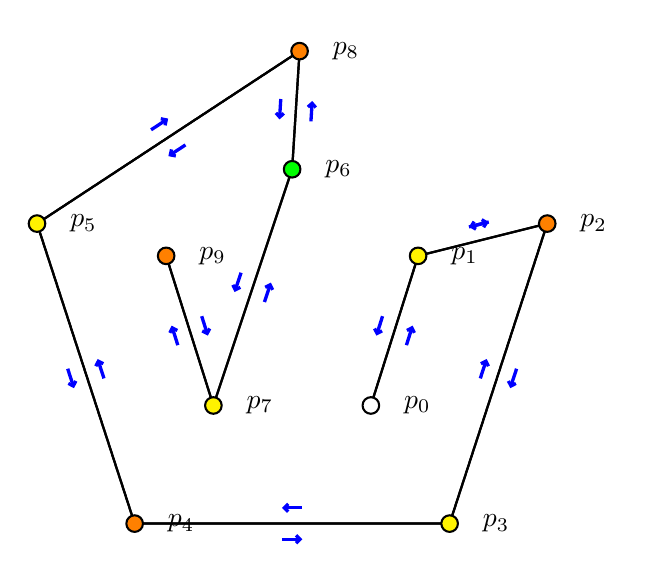
\begin{tikzpicture}[
    start chain = A going right,
pics/AB/.style args = {#1/#2/#3}{code={
    \draw[solid,-{Straight Barb[length=0.5mm]},very thick]
        (-2mm,#1 2mm) -- node [#2,font=\footnotesize,inner sep=0.5pt] {#3} ++ (4mm,0mm);}
                            },
pics/BA/.style args = {#1/#2/#3}{code={
    \draw[solid,{Straight Barb[length=0.5mm]}-,very thick]
        (-2mm,#1 2mm) -- node [#2,font=\footnotesize,inner sep=0.5pt] {#3} ++ (4mm,0mm);}
                            }
                    ]
    \begin{scope}[every node/.style={circle, draw, minimum size=1.5em, 
          inner sep=2pt, on chain}]
%          Vértices:
           % Fig exterior:
           \node(0) [orangeV, label=180:$p_8$] at (1.2, 6)      {};
           \node(1) [orangeV, label=180:$p_2$] at (3.24, 3.81)   {};
           \node(2) [yellowV, label=180:$p_3$] at (2,  0)       {};
           \node(3) [orangeV, label=180:$p_4$] at (-2, 0)       {};
           \node(4) [yellowV, label=180:$p_5$] at (-3.24, 3.81) {};
           % Fig interior:
           \node(5) [greenV, label=180:$p_6$] at (0, 4.5)       {};
           \node(6) [yellowV, label=180:$p_1$] at (1.6,  3.4)   {};
           \node(7) [vertex, label=180:$p_0$] at (1, 1.5)       {};
           \node(8) [yellowV, label=180:$p_7$] at (-1, 1.5)     {};
           \node(9) [orangeV, label=180:$p_9$] at (-1.6, 3.4)   {};
      
%          Aristas:
    \end{scope}
    \begin{scope}[sloped]
\draw[thick]    (0) --  pic [blueE] {BA= - /below right/} (4)
                (0) --  pic [blueE] {BA= /below left/}    (5);

\draw[thick]    (1) --  pic [blueE] {BA= -/below right/} (2)
                (1) --  pic [blueE] {BA= /above left/}   (6);

\draw[thick]    (2) --  pic [blueE] {AB= /above left/}    (1)
                (2) --  pic [blueE] {BA= /above right/}   (3);

\draw[thick]    (3) --  pic [blueE] {AB= - /below left/}  (2)
                (3) --  pic [blueE] {BA= /above right/}   (4);

\draw[thick]    (4) --  pic [blueE] {AB= - /below left/}  (3)
                (4) --  pic [blueE] {AB= /above left/}    (0);

\draw[thick]    (5) --  pic [blueE] {AB= - /below left/}  (0)
                (5) --  pic [blueE] {BA= /above right/}   (8);

\draw[thick]    (6) --  pic [blueE] {AB= /below left/}    (1)
                (6) --  pic [blueE] {BA= /above left/}    (7);

\draw[thick]    (7) --  pic [blueE] {AB= - /below left/}  (6);

\draw[thick]    (8) --  pic [blueE] {AB= -/above left/}    (5)
                (8) --  pic [blueE] {AB= /above right/}    (9);

\draw[thick]    (9) --  pic [blueE] {BA= - /below left/}  (8);
   \end{scope}
\end{tikzpicture}
\end{document}
